\documentclass[11pt]{article}
\usepackage[a4paper,margin=2.5cm]{geometry}
\usepackage{amsmath, amssymb, hyperref}
\usepackage{physics}
\usepackage{slashed}
\usepackage{graphicx}

\title{Lepton Number and Flavor Violation:\
An Effective Field Theory Perspective}
\author{Fabio Elisiario Fioravante}
\date{}

\begin{document}

\maketitle

\section*{Motivation}

The motivation here lies in the fact that the conservation of lepton number and lepton flavor in the Standard Model is a consequence of an accidental symmetry. Unlike gauge symmetries, these symmetries are not imposed a priori, and their violation does not spoil the consistency of the model. Therefore, new interactions that violate lepton number or lepton flavor can arise in theories beyond Standard Model (BSM), and the search for such violations is a way to explore new physics. What we will see is that there are indeed good reasons to place lepton number and flavor violation in BSM models, whether due to neutrino masses, anomalies found in experiments, cosmological issues such as baryon asymmetry or even grand unification theories.

However, the approach we will take here is more agnostic, and does not rely on a specific model, but maps what BSM models can be. For this, we will use the tool of effective field theories, which allows us to find lepton number and flavor violation by looking at operators of dimension greater than 4, which are suppressed by a scale of new physics, and which can be generated by a variety of BSM models.

This document is just a prototype of what will be for the final project of the course, and aims to motivate the seminar, show what will be covered, as well as do an example calculation that will be important for the project. With this goal in mind, in this text we will calculate the process $\mu\rightarrow e +\gamma$, which violates lepton flavor, in Standard Model and then using dimension 6 dipole operators, to show the 'matching' between these two approaches and highlight where new physics can be phenomenologically searched for. 

\section*{$\mu \to e \gamma$}

\begin{figure}[h]
    \centering
    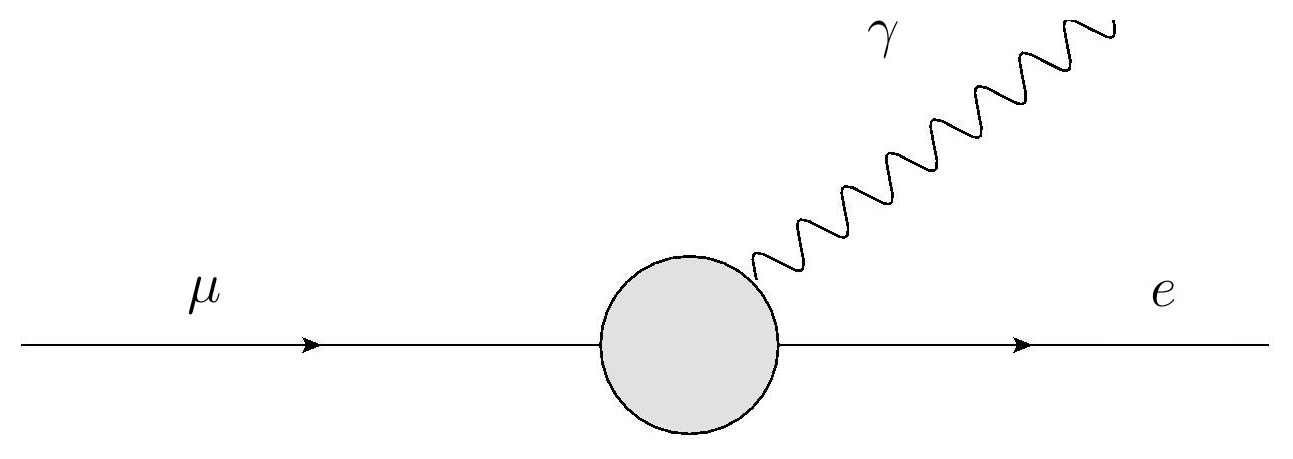
\includegraphics[width=0.65\textwidth]{diagramageral_trim.png}
    \caption{General amplitude for $\mu \to e\gamma$, with the blob representing all possible contributions.}
    \label{fig:diagramageral}
\end{figure}

\subsection*{General calculation}

We consider the radiative charged-lepton flavor violating decay
\begin{equation}
    \mu(p) \to e(p-q) + \gamma(q).
\end{equation}

The amplitude can be written as
\begin{equation}
    \mathcal{M}(\mu \to e\gamma)
    =
     \epsilon^{*\mu}(q)
    \mel{e}{J_\mu^{\rm em}}{\mu},
\end{equation}
we can write the most general matrix element using all possible Lorentz stuctures
\begin{equation}
    \mel{e}{J_\mu^{\rm em}}{\mu}
    =
    \bar{u}_e(p-q)
    \left[
        i q^\nu \sigma_{\mu\nu} (A + B\gamma_5)
        + \gamma_\mu (C + D\gamma_5)
        + q_\mu (E + F\gamma_5)
    \right]
    u_\mu(p).
\end{equation}

From the Ward identity of electromagnetism,
\begin{equation}
    \partial^\mu J_\mu^{\rm em}=0,
\end{equation}
we have
\begin{equation}
    q^\mu \mel{e}{J_\mu^{\rm em}}{\mu}=0.
\end{equation}

Contracting the general decomposition with $q^\mu$, one obtains
\begin{align}
    q^\mu J_\mu^{\rm em}
    &=
    i q^\mu q^\nu \sigma_{\mu\nu}(A+B\gamma_5)
    + \slashed{q}(C+D\gamma_5)
    + q^2(E+F\gamma_5),
\end{align}
and first term vanishes because $q^\mu q^\nu$ is symmetric while
$\sigma_{\mu\nu}$ is antisymmetric:
\begin{equation}
    q^\mu q^\nu \sigma_{\mu\nu}=0.
\end{equation}

Since the external photon is on shell,
\begin{equation}
    q^2=0,
\end{equation}
the Ward identity reduces to
\begin{equation}
    \bar{u}_e(p-q)\slashed{q}(C+D\gamma_5)u_\mu(p)=0.
\end{equation}

Using
\begin{equation}
    q = p - (p-q),
\end{equation}
and the Dirac equations
\begin{equation}
    \slashed{p} u_\mu(p)=m_\mu u_\mu(p),
    \qquad
    \bar{u}_e(p-q)(\slashed{p}-\slashed{q})=m_e \bar{u}_e(p-q),
\end{equation}
we find
\begin{align}
    \bar{u}_e(p-q)\slashed{q}(C+D\gamma_5)u_\mu(p)
    &=
    \bar{u}_e(p-q)
    \left[
        \slashed{p} - (\slashed{p}-\slashed{q})
    \right]
    (C+D\gamma_5)u_\mu(p)
    \notag \\
    &=
    \bar{u}_e(p-q)
    \left[
        m_\mu(C-D\gamma_5)
        -
        m_e(C+D\gamma_5)
    \right]
    u_\mu(p).
\end{align}

Therefore,
\begin{equation}
    m_e(C+D\gamma_5)-m_\mu(C-D\gamma_5)=0.
\end{equation}

In the limit $m_e \ll m_\mu$, this implies
\begin{equation}
    C=D=0.
\end{equation}

Thus the remaining amplitude is
\begin{equation}
    \mathcal{M}(\mu \to e\gamma)
    =
    \epsilon^{*\mu}(q)\,
    \bar{u}_e(p-q)
    \left[
        i q^\nu \sigma_{\mu\nu}(A+B\gamma_5)
    \right]
    u_\mu(p).
    \label{agr}
\end{equation}

Using the chiral projectors
\begin{equation}
    P_{R,L} = \frac{1\pm \gamma_5}{2},
\end{equation}
we can rewrite
\begin{equation}
    A+B\gamma_5 = A_R P_R + A_L P_L,
\end{equation}
where
\begin{equation}
    A_R = A+B,
    \qquad
    A_L = A-B.
\end{equation}

Therefore,
\begin{equation}
    \mathcal{M}(\mu \to e\gamma)
    =
    \epsilon^{*\mu}(q)\,
    \bar{u}_e(p-q)
    i\sigma_{\mu\nu}q^\nu
    \left(
        A_R P_R + A_L P_L
    \right)
    u_\mu(p).
\end{equation}

After summing over final spins and photon polarizations, and averaging over the initial muon spin, using mathematica, one obtains
\begin{equation}
    \overline{|\mathcal{M}|^2}
    =
    m_\mu^4 
    \left(
        |A_R|^2 + |A_L|^2
    \right),
\end{equation}
where we have used $m_\mu \gg m_e$.

The decay width is then
\begin{equation}
    \Gamma(\mu \to e\gamma)
    =
    \frac{1}{16\pi m_\mu}
    \overline{|\mathcal{M}|^2}
    =
    \frac{m_\mu^3 }{16\pi}
    \left(
        |A_R|^2 + |A_L|^2
    \right).
\end{equation}

\begin{figure}[h]
    \centering
    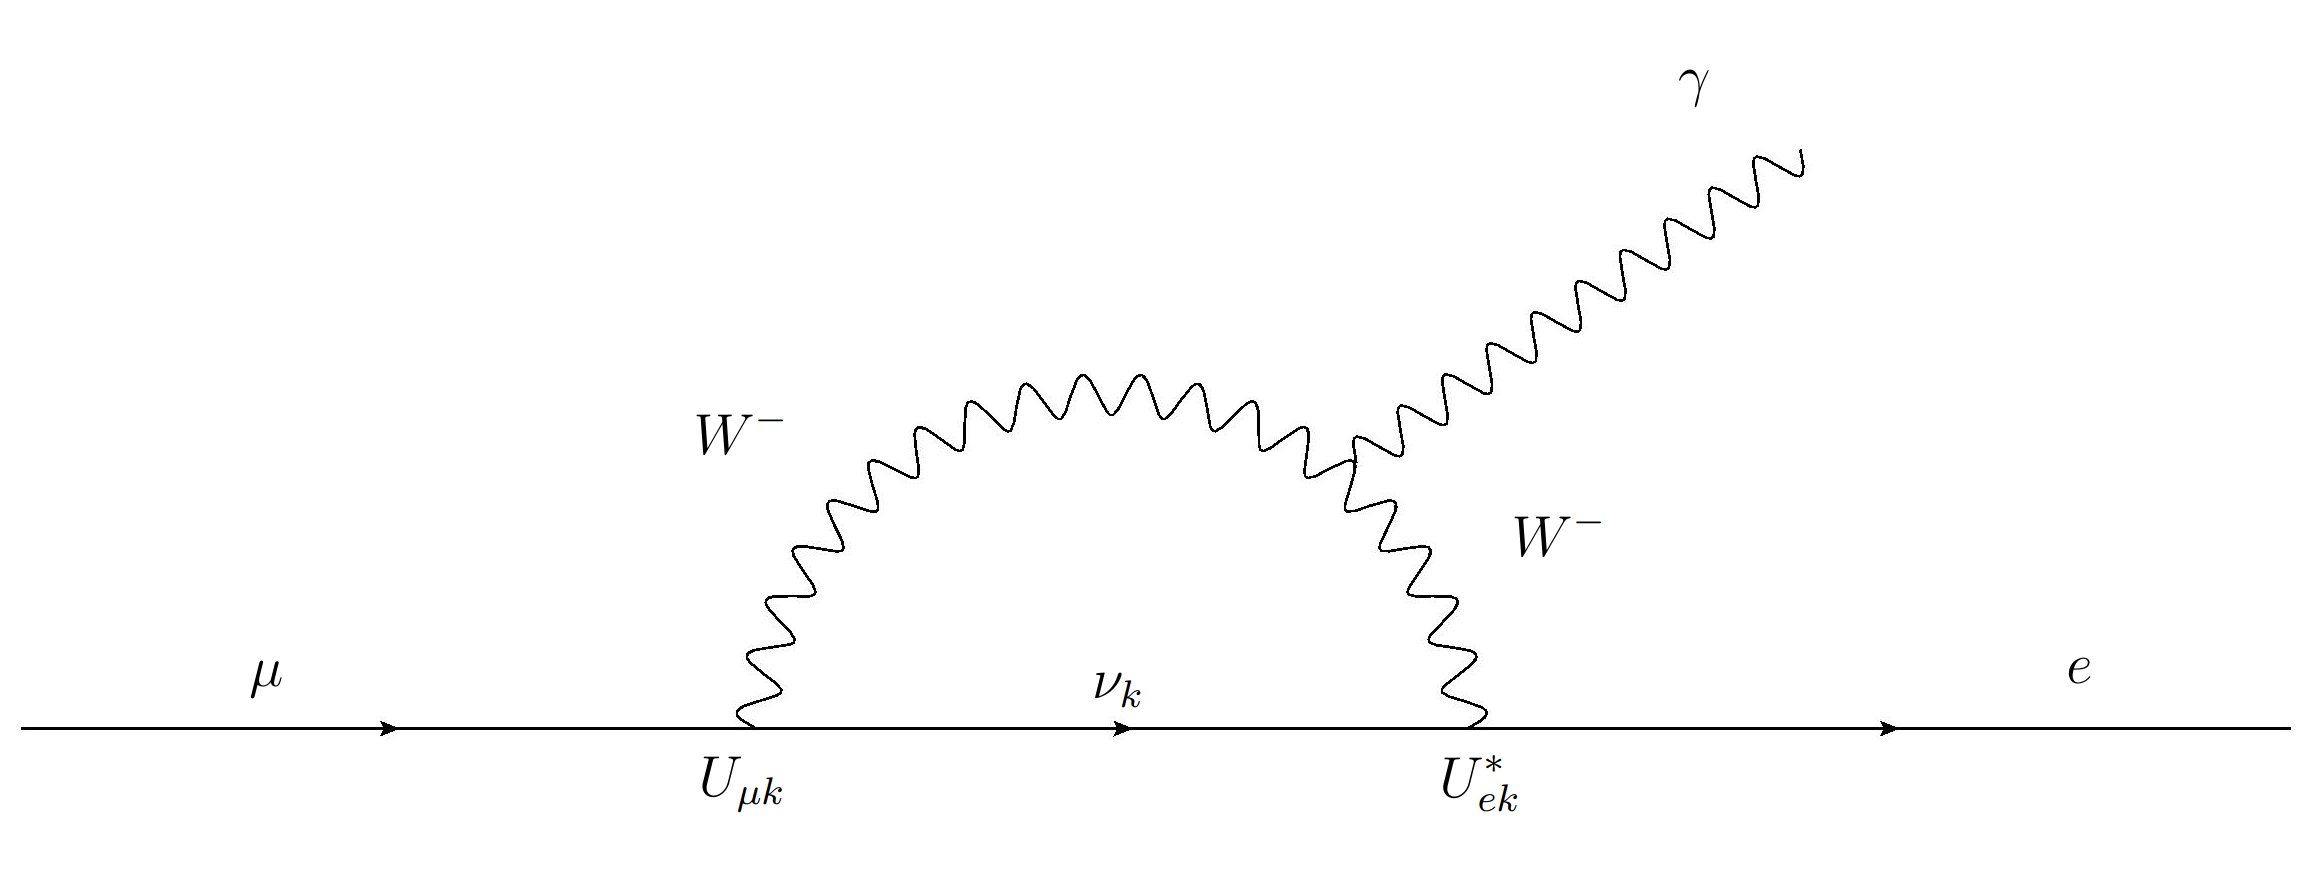
\includegraphics[width=0.65\textwidth]{diagramcerto_trim.png}
    \caption{One-loop diagram contributing to $\mu \to e\gamma$ in the SM.}
    \label{fig:diagram}
\end{figure}

\subsection*{SM calculation}

We now compute the contribution in the Standard Model with massive neutrinos. Working in $R_\xi$ gauge and neglecting Goldstone bosons, the relevant diagram contains a $W$ boson and a neutrino running in the loop.


The one-loop amplitude is, by Fig.~\ref{fig:diagram}
\begin{align}
    i\mathcal{M}^{(1)}
    &=
    \int \frac{d^4k}{(2\pi)^4}\,
    \bar{u}_e(p-q)
    \sum_k
    \frac{g}{\sqrt{2}} U^*_{ek}
    \gamma^\alpha
    \frac{1-\gamma_5}{2}
    \frac{i(\slashed{p}-\slashed{k}+m_{\nu_k})}
    {(p-k)^2-m_{\nu_k}^2}
    \frac{g}{\sqrt{2}} U_{\mu k}
    \gamma^\beta
    \frac{1-\gamma_5}{2}
    u_\mu(p)
    \notag \\
    &\quad \times
    \frac{-i}{k^2-m_W^2}
    \left(
        g_{\alpha\rho}
        -
        (1-\xi)\frac{k_\alpha k_\rho}{k^2-\xi m_W^2}
    \right)
    \left[
        -ie\,\Gamma^{\rho\sigma\mu}_{WW\gamma}
    \right]
    \notag \\
    &\quad \times
    \frac{-i}{(k+q)^2-m_W^2}
    \left(
        g_{\sigma\beta}
        -
        (1-\xi)\frac{(k+q)_\sigma (k+q)_\beta}
        {(k+q)^2-\xi m_W^2}
    \right)
    \epsilon^*_\mu(q).
\end{align}

Where $ \Gamma_{\rho\sigma\mu}^{WW\gamma}$ is the three-gauge-boson vertex content,
\begin{equation}
    \Gamma_{\rho\sigma\mu}^{WW\gamma}
    =
    (-q-k)_\sigma g_{\rho\mu}
    +
    (2k+q)_\mu g_{\rho\sigma}
    -
    (2q+k)_\rho g_{\sigma\mu}.
\end{equation}

The fermionic propagator can be expanded as
\begin{equation}
    \sum_k
    \frac{U_{\mu k}U^*_{ek}}
    {(p-k)^2-m_{\nu_k}^2}
    =
    \sum_k
    \left[
        \frac{U_{\mu k}U^*_{ek}}{(p-k)^2}
        +
        \frac{U_{\mu k}U^*_{ek}m_{\nu_k}^2}{(p-k)^4}
        + \cdots
    \right].
\end{equation}

Using unitarity of the PMNS matrix,
\begin{equation}
    UU^\dagger = 1,
\end{equation}
we have
\begin{equation}
    \sum_k U_{\mu k}U^*_{ek} = \delta_{\mu e}=0.
\end{equation}

Therefore the leading term vanishes, and the first surviving contribution is proportional to
\begin{equation}
    \sum_k U_{\mu k}U^*_{ek}m_{\nu_k}^2.
\end{equation}

Using, again, the unitarity of the PMNS matrix, this can also be written as
\begin{align}
    \sum_k U_{\mu k}U^*_{ek}m_{\nu_k}^2
    &=
    -m_1^2
    \left(
        U_{\mu 2}U^*_{e2}
        +
        U_{\mu 3}U^*_{e3}
    \right)
    +
    U_{\mu 2}U^*_{e2}m_2^2
    +
    U_{\mu 3}U^*_{e3}m_3^2
    \notag \\
    &=
    U_{\mu 2}U^*_{e2}\Delta m_{21}^2
    +
    U_{\mu 3}U^*_{e3}\Delta m_{31}^2.
\end{align}

This means that differences of neutrino masses are responsible for the amount of charged lepton flavor violation generated in the SM, that is, the suppression
for charged lepton flavor violating, are originated by small neutrino mass differences. In the left-handed part amplitude, however, the suppression is even stronger because of the chirality structure. \eqref{agr} shows that the external $\mu$ and $e$ must to have opposite chiralities and, since the loop is generated by left handed current, there will be have a chirality flip for one of the external legs, that is proportional to the mass of the lepton.

For the dominant amplitude, the loop calculation gives
\begin{equation}
    A^{(1)}_R
    =
    \frac{g^2\ e}{128\pi^2}
    \frac{m_\mu}{m_W^4}
    \sum_{k=2,3}
    U_{\mu k}U^*_{ek}m_{\nu_k}^2
    \left[1
        -\frac{1}{3}\frac{\ln\xi}{\xi-1}
        +
        \frac{1}{\xi-1}
        \left(
            \frac{\xi\ln \xi}{\xi-1}
            -1
        \right)
    \right].
    \label{AR}
\end{equation}

Here $\xi$ denotes the gauge parameter associated with the $R_\xi$ gauge calculation.

Here we got a apparently gauge dependent result, but this is not the case, so I think it would be useful to include a brief discussion about the choice of gauge in this case. In the beginning of the calculation, we state that we are working in the $R_\xi$ gauge, and we neglect the contribution of the Goldstone bosons of electroweak symmetry breaking, in fact there are diagrams with Goldstone bosons contributing to the amplitude, and we can see their role separating 2 ways of doing the calculation. 

If we do the calculation in an arbitrary $R_\xi$ gauge, we have to include the contribution of the Goldstone bosons, and their contribution will exactly cancel the gauge dependent part of Eq.~\eqref{AR}, yielding to a gauge independent result. On the other hand if we do the calculation in the unitary gauge, that is take $\xi\to\infty$ in Eq.~\eqref{AR}, the result does not depend on $\xi$ anymore, and this represent the case where the Goldstone bosons decouple from the theory, and therefore do not contribute to the amplitude. As expected, both approaches give the same result.

Taking the limit $\xi \to \infty$, that is the unitary gauge, the loop function tends to
\begin{equation}
    A_R^{(1)} \to A_R.
\end{equation}

The loop calculation (in unitary gauge) was performed using Mathematica. The result is consistent with the literature, and can be found in \cite{cheng_li_gauge} and \cite{Calibbi2018}



Thus the branching ratio behaves as
\begin{equation}
    BR(\mu\to e \gamma)=\frac{\Gamma(\mu \to e\gamma)}{\Gamma(\mu \to e\nu\bar\nu)}
    \propto
    \left|
        \sum_{k=2,3}
        U_{\mu k}U^*_{ek}
        \frac{\Delta m_{k1}^2}{m_W^2}
    \right|^2
    \sim 10^{-47},
\end{equation}

assuming the literature values for $\Gamma(\mu\to e\nu\bar\nu)=m_\mu^5 G_F^2/(192\pi^3)$ and $\Delta m_{21}^2 \approx 7.50\times 10^{-5}\,\text{eV}^2$ and $\Delta m_{31}^2 \approx 2.46\times 10^{-3}\,\text{eV}^2$. 

\subsection*{EFT calculation}

At the effective-field-theory level, the leading contribution to $\mu \to e\gamma$ comes from dimension-six dipole operators. The relevant terms in the effective Lagrangian are
\begin{equation}
    \mathcal{L}
    \supset
    \frac{C^{e\gamma}_{e\mu}}{\Lambda^2}
    \frac{v}{\sqrt{2}}\,
    \bar{e}\sigma_{\mu\nu}P_R\mu\,F^{\mu\nu}
    +
    \frac{C^{e\gamma}_{\mu e}}{\Lambda^2}
    \frac{v}{\sqrt{2}}\,
    \bar{\mu}\sigma_{\mu\nu}P_R e\,F^{\mu\nu}
    + \text{h.c.},
\end{equation}
where $v$ is the vacuum expectation value of the Higgs field, $\Lambda$ is the 'cutoff' of Standard Model, and $C^{e\gamma}_{e\mu}$ and $C^{e\gamma}_{\mu e}$ are dimensionless Wilson coefficients, that parametrize our ignorance about the underlying new physics. Notice that this vertex is valid in the energy regime between the electroweak scale, say $\sim m_W \sim 100$ GeV, and the scale $\Lambda$ of new physics, so we must assume $\Lambda \gg m_W$.

Equivalently, after taking the hermitian conjugate of the second term, the amplitude can be written as
\begin{equation}
    i\mathcal{M}
    =
    \bar{u}_e(p-q)
    \frac{v}{\sqrt{2}\Lambda^2}
    \sigma_{\mu\nu}q^\mu
    \left[
        C^{e\gamma}_{e\mu}P_R
        +
        C^{e\gamma *}_{\mu e}P_L
    \right]
    u_\mu(p)\,
    \epsilon^{*\nu}(q).
\end{equation}

Matching this amplitude with the general parametrization,
\begin{equation}
    \mathcal{M}(\mu \to e\gamma)
    =
    \epsilon^{*\mu}
    \bar{u}_e i\sigma_{\mu\nu}q^\nu
    \left(
        A_RP_R+A_LP_L
    \right)
    u_\mu,
\end{equation}
we identify
\begin{equation}
    C^{e\gamma}_{e\mu}
    =
    A_R \frac{\sqrt{2}\Lambda^2 e}{v},
    \qquad
    C^{e\gamma *}_{\mu e}
    =
    A_L \frac{\sqrt{2}\Lambda^2 e}{v}.
\end{equation}

Therefore,
\begin{equation}
    A_R =
    \frac{v}{\sqrt{2}\Lambda^2}
    C^{e\gamma}_{e\mu},
    \qquad
    A_L =
    \frac{v}{\sqrt{2}\Lambda^2}
    C^{e\gamma *}_{\mu e}.
\end{equation}

Substituting into the decay width,
\begin{equation}
    \Gamma(\mu \to e\gamma)
    =
    \frac{m_\mu^3 }{16\pi}
    \left(
        |A_R|^2+|A_L|^2
    \right),
\end{equation}
we obtain
\begin{equation}
    \Gamma(\mu \to e\gamma)
    =
    \frac{m_\mu^3 v^2}{32\pi\Lambda^4}
    \left(
        |C^{e\gamma}_{e\mu}|^2
        +
        |C^{e\gamma}_{\mu e}|^2
    \right).
\end{equation}

\subsection*{Matching SM to EFT}

Equating the SM one-loop result in the unitary gauge with the EFT expression $A_R = \frac{v}{\sqrt{2}\Lambda^2}C^{e\gamma}_{e\mu}$, we can read off the Wilson coefficient that the SM generates, in energy scales around the electroweak scale:
\begin{equation}
    \frac{C^{e\gamma}_{e\mu}}{\Lambda^2}\bigg|_{\rm \mu\sim 100\,\text{GeV}}
    =
    \frac{\sqrt{2}}{v}
    \cdot
    \frac{g^2 e}{128\pi^2}
    \frac{m_\mu}{m_W^4}
    \sum_{k=2,3}
    U_{\mu k}U^*_{ek}m_{\nu_k}^2.
    \label{eq:matching}
\end{equation}
 
We can see that the effective coupling is suppressed by $m_\nu^2/m_W^4$ which will result in $\text{BR}(\mu\to e\gamma)\sim 10^{-47}$ in the SM. On the other hand, a generic BSM theory at scale $\Lambda$ generates $C^{e\gamma}_{e\mu}/\Lambda^2 \sim 1/\Lambda^2$ for $C = \mathcal{O}(1)$, changing the branching ratio to values accessible to current experiments for $\Lambda \sim \mathcal{O}(\text{TeV})$, with the experimental limit $\text{BR}(\mu\to e\gamma) < 1.5\times 10^{-13}$ (MEG II) \cite{meg}.



\section*{What can be done in the final project}

The final project will start with a motivation of the search for lepton number and flavor violation, followed by a quick review of neutrino masses and mixing and effective field theories. Then, the next logical step will be to comment the weinberg operator, which is the unique dimension 5 operator that violates lepton number (lepton flavor at loop level), and its connection with neutrino masses.

After that, we can move to explicit cases of LNV and LFV, and the $\mu\to e\gamma$ process is a good example of LFV, there are much more things to comment about this process, while neutrinoless double beta decay is a good example of LNV, and we can also comment about the connection between these two processes, and how they are natural pathways to some new physics models, such as seesaw, left-right symmetric models, leptoquarks, etc.

Finally, we choose, unlike choosing a specific model, to do an EFT approach to the processes, and comment about the operators that can generate LNV and LFV, and the phenomenological gain (and loss) of this approach, and how it can be used to constrain BSM models.

\section*{Acknowledgments}
I would like to thank Luighi Leal for the fruitful discussions on the subtleties of the subject and calculation, and for the assistance with the Wolfram Mathematica code for the loop integral.
\nocite{*}
\bibliographystyle{unsrt}
\bibliography{referencias}


\end{document}
